\documentclass[a4paper,11pt]{article}

\usepackage[portuguese]{babel}
\usepackage[utf8]{inputenc}
\usepackage{amsmath}
\usepackage{graphicx}
\usepackage{hyperref}
\usepackage{float}
\usepackage{subfig}
\usepackage{fixltx2e}
\usepackage[bottom]{footmisc}
\usepackage{listings}
\usepackage{xargs}                      % Use more than one optional parameter in a new commands
\usepackage[pdftex,dvipsnames]{xcolor}  % Coloured text etc.
\usepackage[colorinlistoftodos,prependcaption,textsize=tiny]{todonotes}
\newcommandx{\unsure}[2][1=]{\todo[linecolor=red,backgroundcolor=red!25,bordercolor=red,#1]{#2}}
\newcommandx{\change}[2][1=]{\todo[linecolor=blue,backgroundcolor=blue!25,bordercolor=blue,#1]{#2}}
\newcommandx{\info}[2][1=]{\todo[linecolor=OliveGreen,backgroundcolor=OliveGreen!25,bordercolor=OliveGreen,#1]{#2}}
\newcommandx{\improvement}[2][1=]{\todo[linecolor=Plum,backgroundcolor=Plum!25,bordercolor=Plum,#1]{#2}}
\newcommandx{\thiswillnotshow}[2][1=]{\todo[disable,#1]{#2}}
\usepackage[font=footnotesize]{caption}
\usepackage[hypcap]{caption}
\usepackage[top=2.5cm, bottom=2.5cm, left=2.5cm, right=2.5cm]{geometry}
\usepackage{enumerate}
%\usepackage[siunitx,american]{circuitikz}

\setcounter{tocdepth}{3}
\setcounter{secnumdepth}{4}

\numberwithin{equation}{section}
\addto\captionsportuguese{\renewcommand{\contentsname}{Índice}}

\linespread{1.3}
\usepackage{indentfirst}

\begin{document}
\begin{titlepage}
\begin{center}

\hfill \break
\hfill \break


\includegraphics[width=0.3\textwidth]{img/logo}~\\[1cm] 

\textsc{\LARGE Instituto Superior Técnico}\\[0.25cm]
\textsc{\Large Mestrado Integrado em Engenharia Electrotécnica e de Computadores}\\[1.8cm]
\textsc{\huge Electrónica de Potência}\\[0.25cm]

\vspace{6mm}

{\huge \bfseries Conversor CC/CC \\[0.7cm]}
{\bfseries Redutor, Ampliador \& Redutor-Ampliador \\[1cm]}

\begin{tabular}{ l l }
	João Bernardo Sequeira de Sá & \hspace{2mm} n.º 68254 \\
	Maria Margarida Dias dos Reis & \hspace{2mm} n.º 73099 \\
	Rafael Augusto Maleno Charrama Gonçalves & \hspace{2mm} n.º 73786 \\
	Nuno Miguel Rodrigues Machado & \hspace{2mm} n.º 74236
\end{tabular}

\vspace{7mm}

Turno de Segunda-feira das 17h00 - 20h00

\vfill

{\large Lisboa,  de Novembro de 2015} 
	
\end{center}
\end{titlepage}
	
\tableofcontents
\pagebreak

\section{Introdução}

O objetivo deste trabalho é estudar o funcionamento das três principais topologias de conversores CC/CC, sendo estas o conversor redutor, conversor ampliador e redutor-ampliador.

Este tipo de conversores pode ser visto como o equivalente em corrente continua de um transformador cuja relação de transformação é variável. Quer isto dizer que através de um conversor CC/CC é possível converter uma certa fonte de tensão continua com valor fixo para uma fonte de tensão com valor variável, fazendo-se uma elevação ou redução do valor. \cite{Rashid}

Sendo assim pode considerar-se que este trabalho está dividido em três partes sendo que em cada uma destas se estuda o funcionamento de uma topologia diferente.

A primeira topologia a considerar é o conversor redutor. O objetivo neste caso é obter-se à saída uma tensão inferior à de entrada, sendo que se pode controlar esta diferença através do fator de ciclo.

De seguida estuda-se o conversor ampliador, onde o objetivo é o contrário da anterior topologia, querendo-se obter à saída uma tensão superior à de entrada. Novamente esta relação pode ser controlada através do fator de ciclo.

Por fim tem-se o conversor redutor-ampliador, onde é possível obter na saída um valor inferior ou superior da tensão de entrada. Novamente o parâmetro de controlo aqui é o fator de ciclo, onde abaixo de um certo valor se obtém uma redução da tensão e acima uma ampliação desta. Em condições de operação semelhantes este conversor não consegue obter uma redução de tensão tão grande quanto o conversor redutor e o mesmo pode ser dito entre a ampliação e o conversor ampliador.


\section{Condução do Trabalho}

\subsection{Conversor Redutor}

\subsubsection{Carga R}

No estudo do conversor redutor começa-se por considerar uma carga resistiva pura, sendo o circuito considerado apresentado na \autoref{fig:Red_R}

\begin{figure}[h]
	\centering
	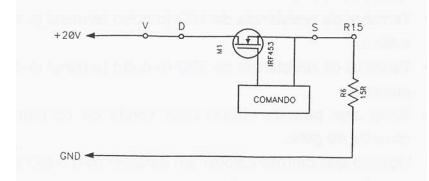
\includegraphics[keepaspectratio=true, scale=0.8]{teoricas/Redutor_R}
	\caption{Esquema do Conversor Redutor com Carga Resistiva.}
	\label{fig:Red_R}
	\vspace{-0.8em}
\end{figure}

	Após feitas as ligações necessárias, regula-se o Gerador de Funções para que se obtenha o sinal quadrado com as caraterísticas desejadas e alimenta-se o circuito de \textit{Drive} e potência tal como indicado no guião.
	
\paragraph{Formas de onda da tensão V\textsubscript{GA} e corrente de \textit{Gate} para $50$ kHz}\mbox{}\

As forma de onda para a tensão V\textsubscript{GA} e corrente de \textit{Gate} podem ser observadas na \autoref{fig:tensao_corrente_gate_buckR}.

\begin{figure}[h]
	\centering
	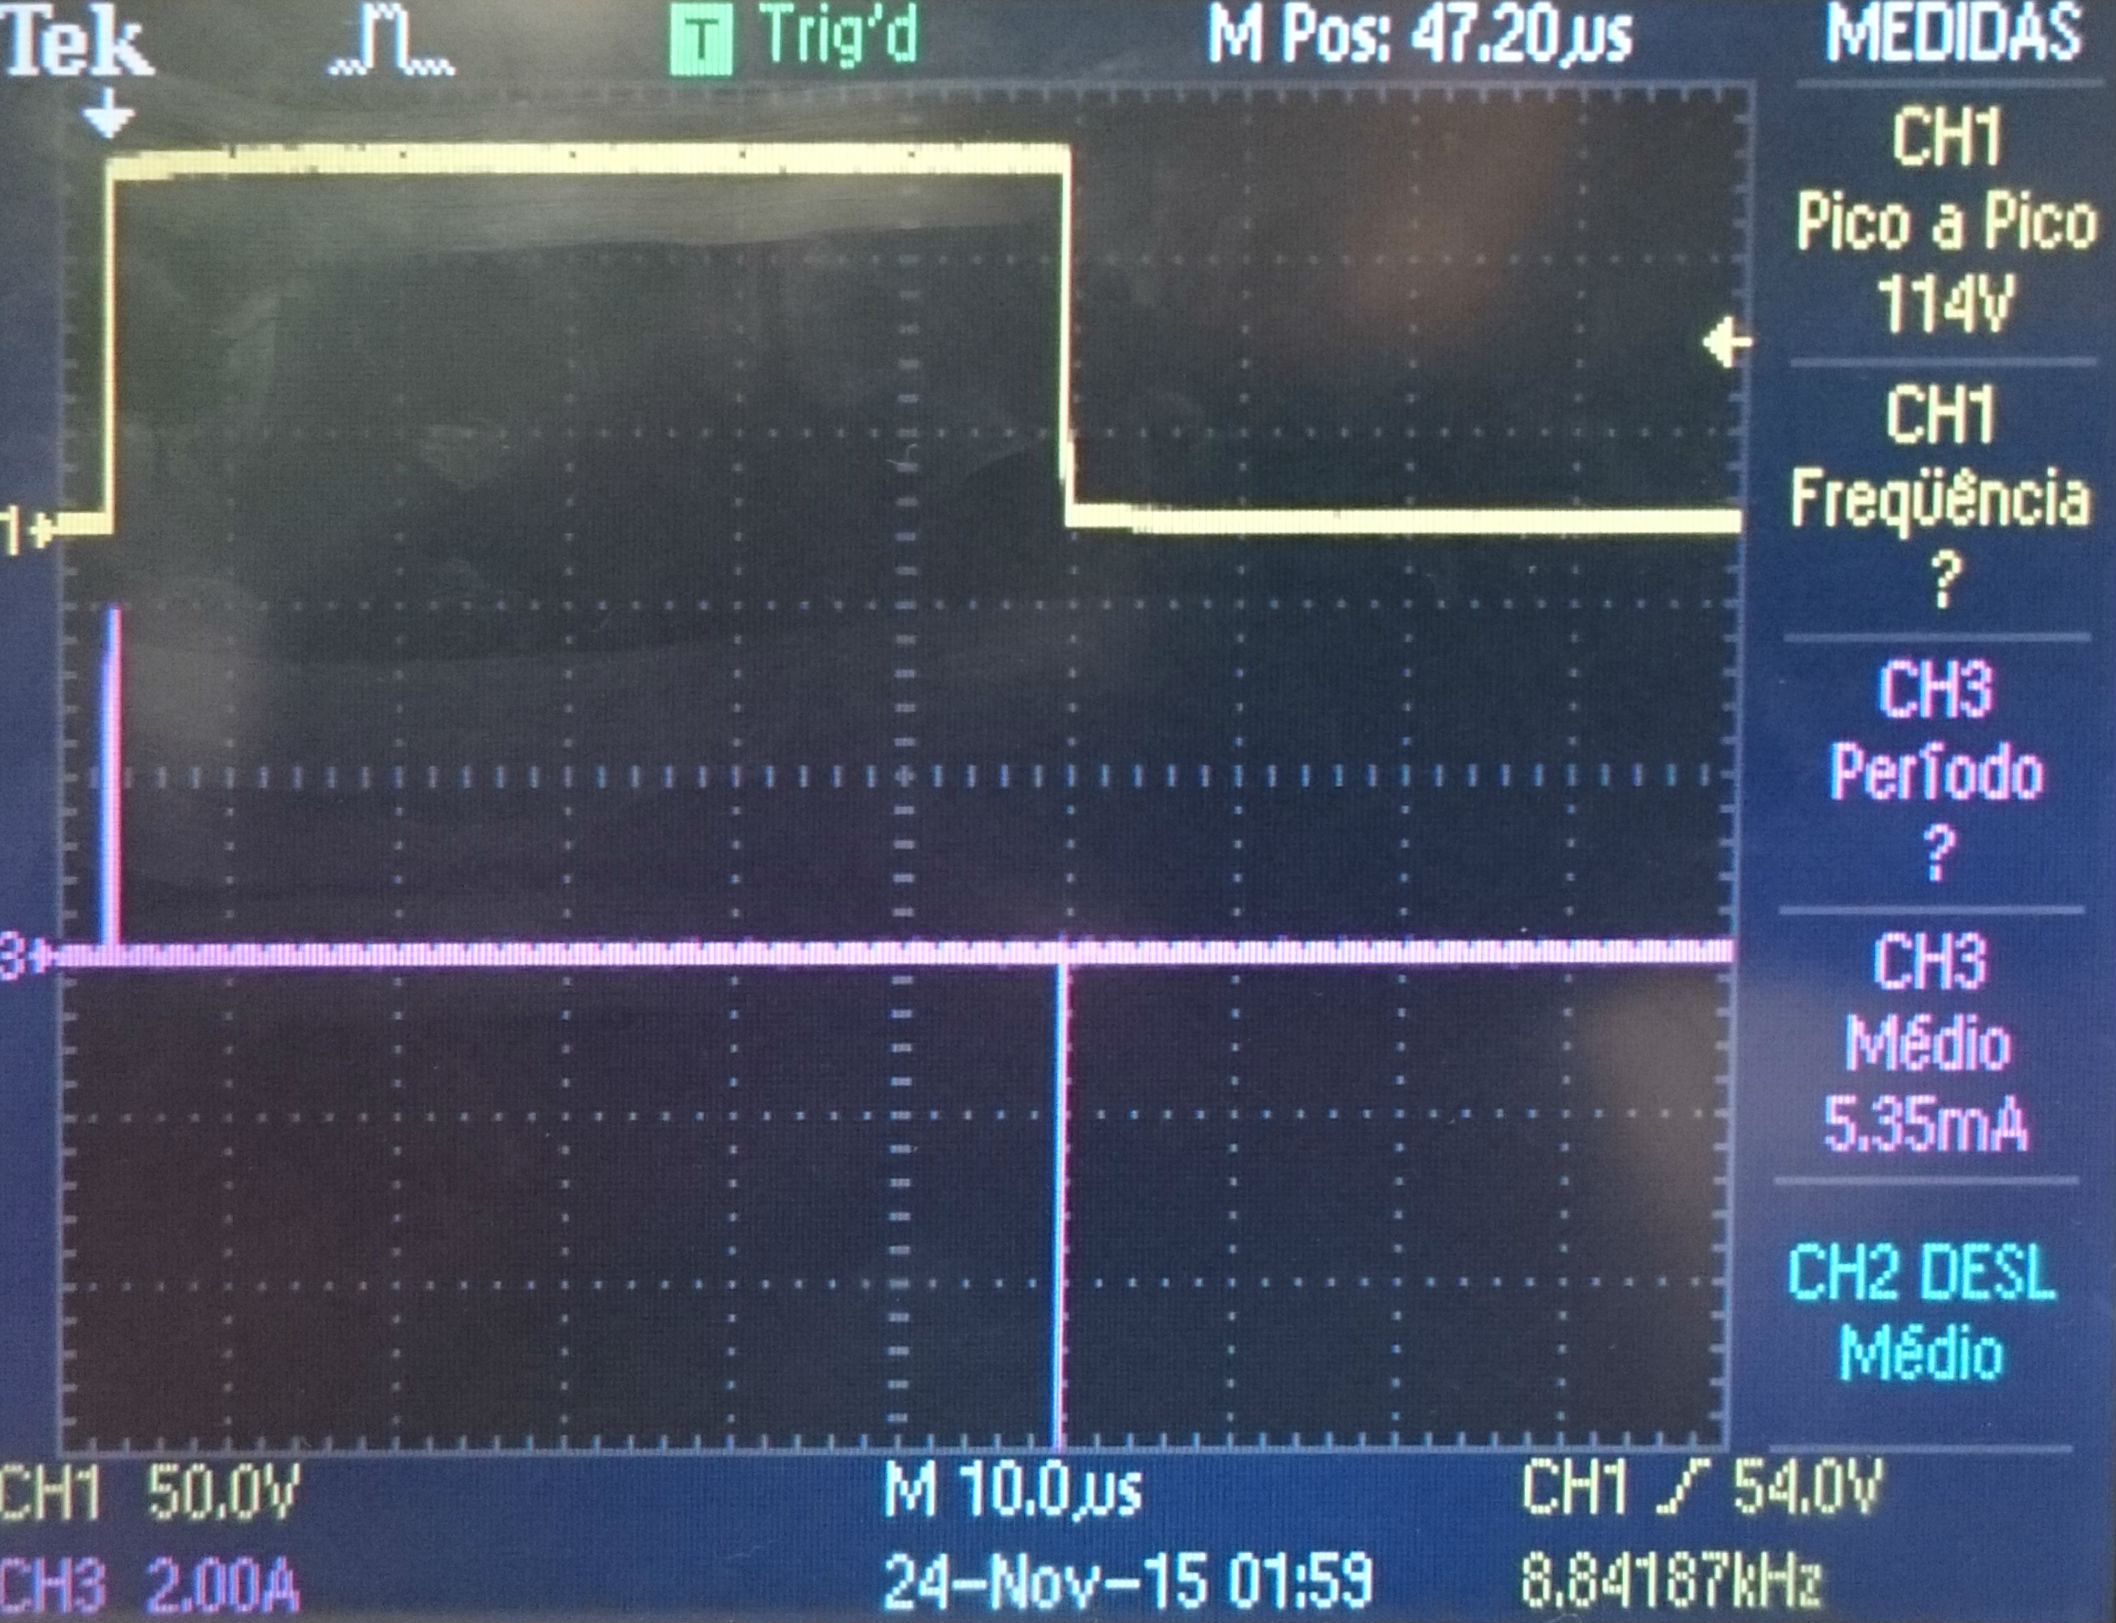
\includegraphics[keepaspectratio=true, scale=0.13]{img/figs/tensao_corrente_gate_buckR}
	\caption{Formas de onda da tensão V\textsubscript{GA} e corrente de \textit{Gate} para Carga Resistiva do conversor Redutor.}
	\label{fig:tensao_corrente_gate_buckR}
	\vspace{-0.8em}
\end{figure} 

Para observar melhor a passagem à condução do transistor MOSFET e o consequente pico de corrente, reduziu-se a escala de tempo sendo o obtido apresentado na \autoref{fig:tensao_corrente_gate_buckR_zoom}.

\begin{figure}[h]
	\centering
	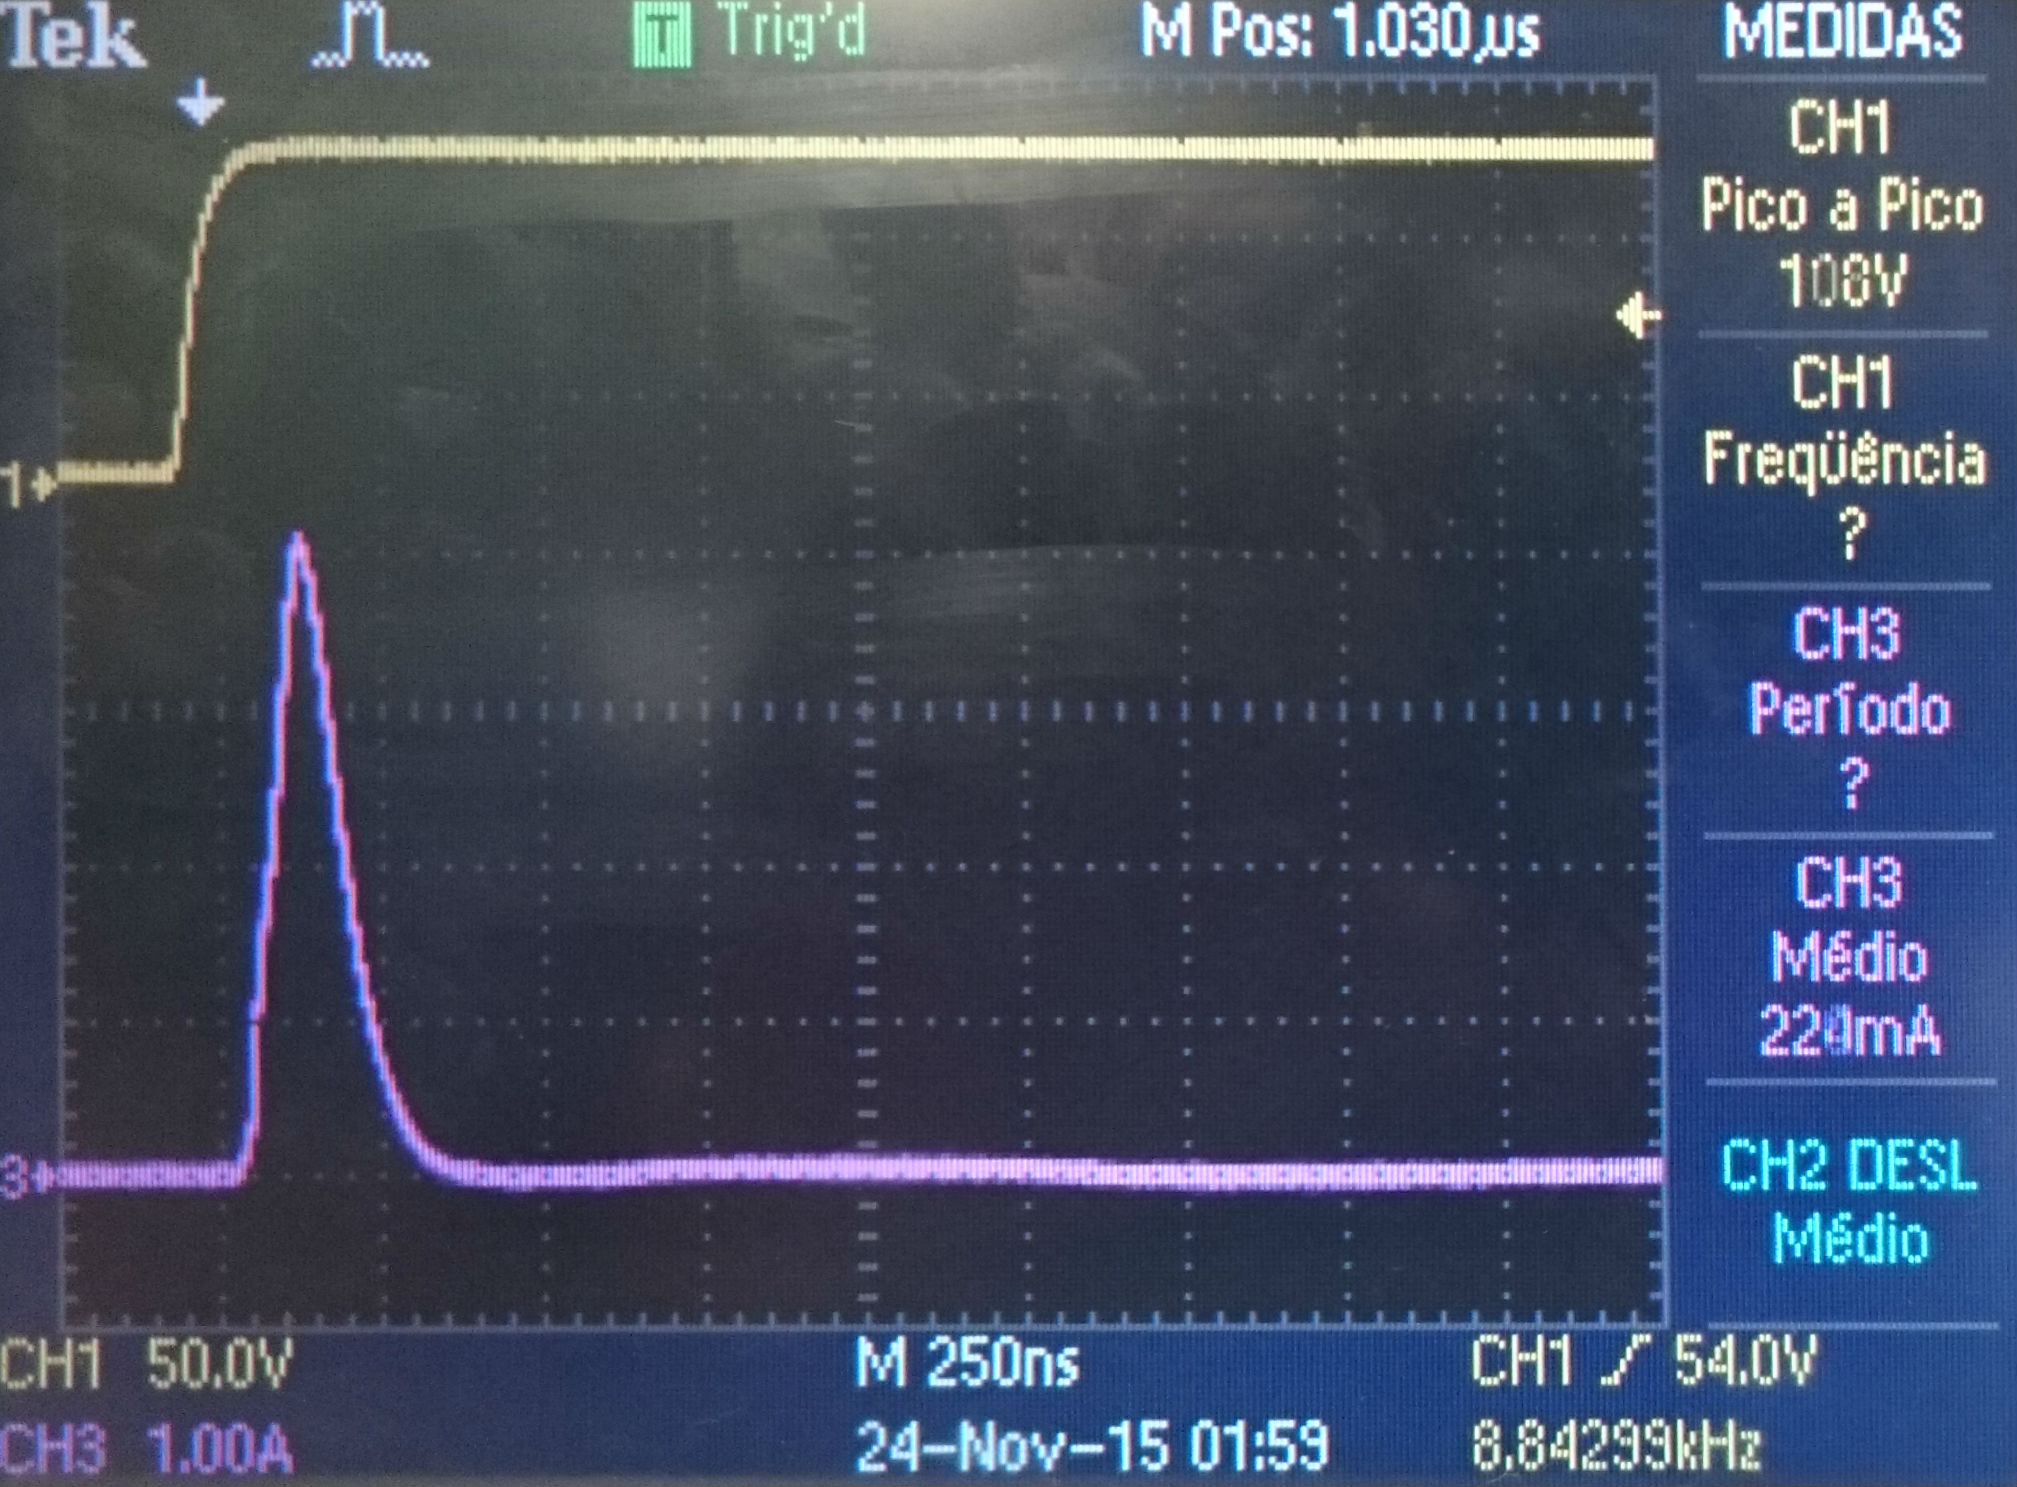
\includegraphics[keepaspectratio=true, scale=0.13]{img/figs/tensao_corrente_gate_buckR_zoom}
	\caption{Formas de onda da tensão V\textsubscript{GA} e corrente de \textit{Gate} para Carga Resistiva do conversor Redutor.}
	\label{fig:tensao_corrente_gate_buckR_zoom}
	\vspace{-0.8em}
\end{figure} 

Em ambas as imagens tem-se a amarelo a tensão V\textsubscript{GA} e a rosa a corrente de \textit{Gate}.

\paragraph{Formas de onda da tensão e corrente na carga}\mbox{}\

De seguida observaram-se as formas de tensão e corrente na carga, estando o obtido presente na \autoref{fig:tensao_corrente_carga_buckR}.

\begin{figure}[h]
	\centering
	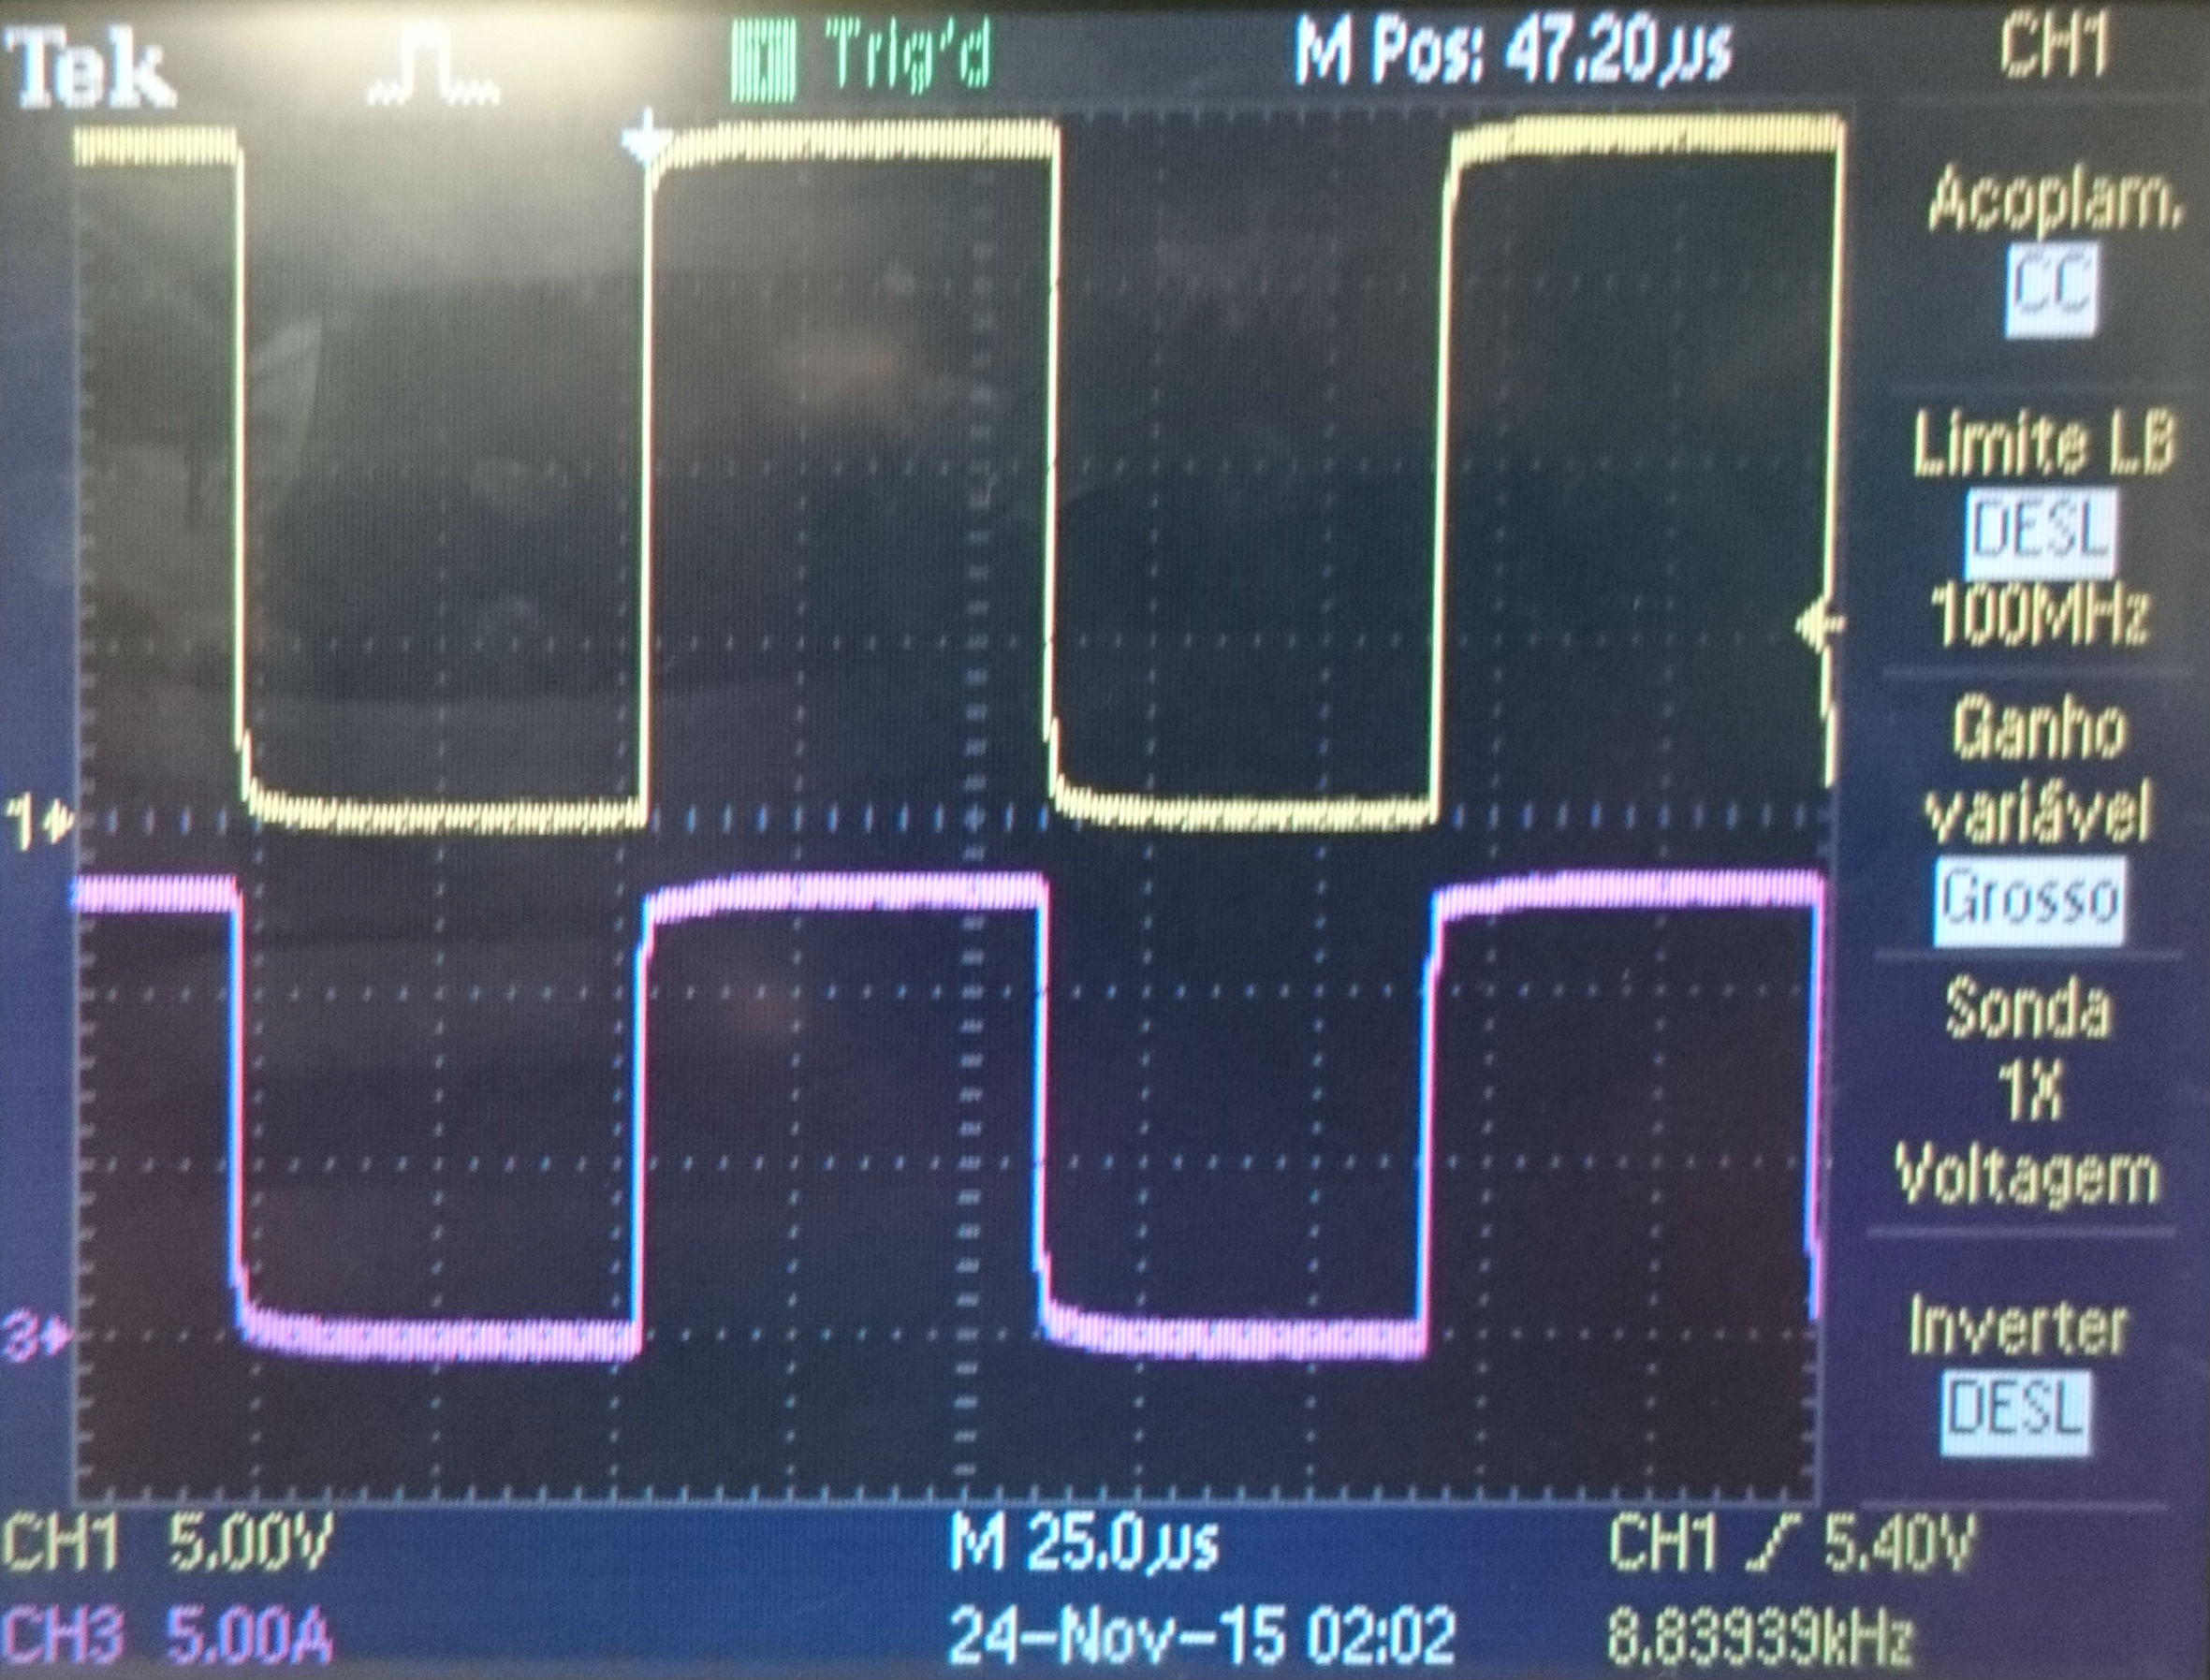
\includegraphics[keepaspectratio=true, scale=0.13]{img/figs/tensao_corrente_carga_buckR}
	\caption{Formas de onda da tensão e corrente na saída para Carga Resistiva do conversor Redutor.}
	\label{fig:tensao_corrente_carga_buckR}
	\vspace{-0.8em}
\end{figure} 

A tensão está apresentada a amarelo e a rosa tem-se a corrente.

A partir da \autoref{fig:tensao_corrente_carga_buckR} e \autoref{fig:tensao_corrente_gate_buckR} pode compreender-se bem o funcionamento deste conversor.

Nota-se que a tensão de saída tem um valor inferior ao de entrada, tendo sido lido $114$ V para a entrada e aproximadamente $20$ V na carga, estando o conversor a reduzir efetivamente a tensão, tal como desejado. Estando-se a trabalhar com uma carga puramente resistiva, não existe qualquer desfasagem entre tensão e corrente na carga, sendo que esta apenas existe quando o transistor MOSFET está à condução.

Observa-se que a tensão na carga não é, no entanto, uma forma quadrada perfeita tal como seria desejado. Isto é provocado por se estar a trabalhar a uma frequência de $50$ kHz, demasiado elevada para que o MOSFET não apresente qualquer atraso. 

As principais fontes para este erro são as componentes incrementais que representam a não idealidade deste componente, pelo que a frequência de operação será limitada.

\subsubsection{Carga RL}

De seguida coloca-se uma bobine em série com a resistência na saída para que se possa estudar o comportamento do circuito a uma carga RL.

O esquema equivalente para este funcionamento está na \autoref{fig:Carga_RL_Buck}

\begin{figure}[h]
	\centering
	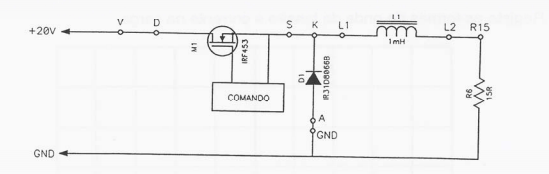
\includegraphics[keepaspectratio=true, scale=0.8]{teoricas/Carga_RL_Buck}
	\caption{Esquema do Conversor Redutor com Carga RL.}
	\label{fig:Carga_RL_Buck}
	\vspace{-0.8em}
\end{figure}

\paragraph{Formas de onda da tensão no Díodo D\textsubscript{1} e corrente na carga para $10$ kHz}\mbox{}\

Após feitas as alterações ao circuito e reduzida a frequência de trabalho para $10$ kHz foram observadas as formas de onda da tensão no díodo D\textsubscript{1} e corrente na carga, sendo o obtido presente na \autoref{fig:tensao_diodo_icarga_buckrl}.

\begin{figure}[H]
	\centering
	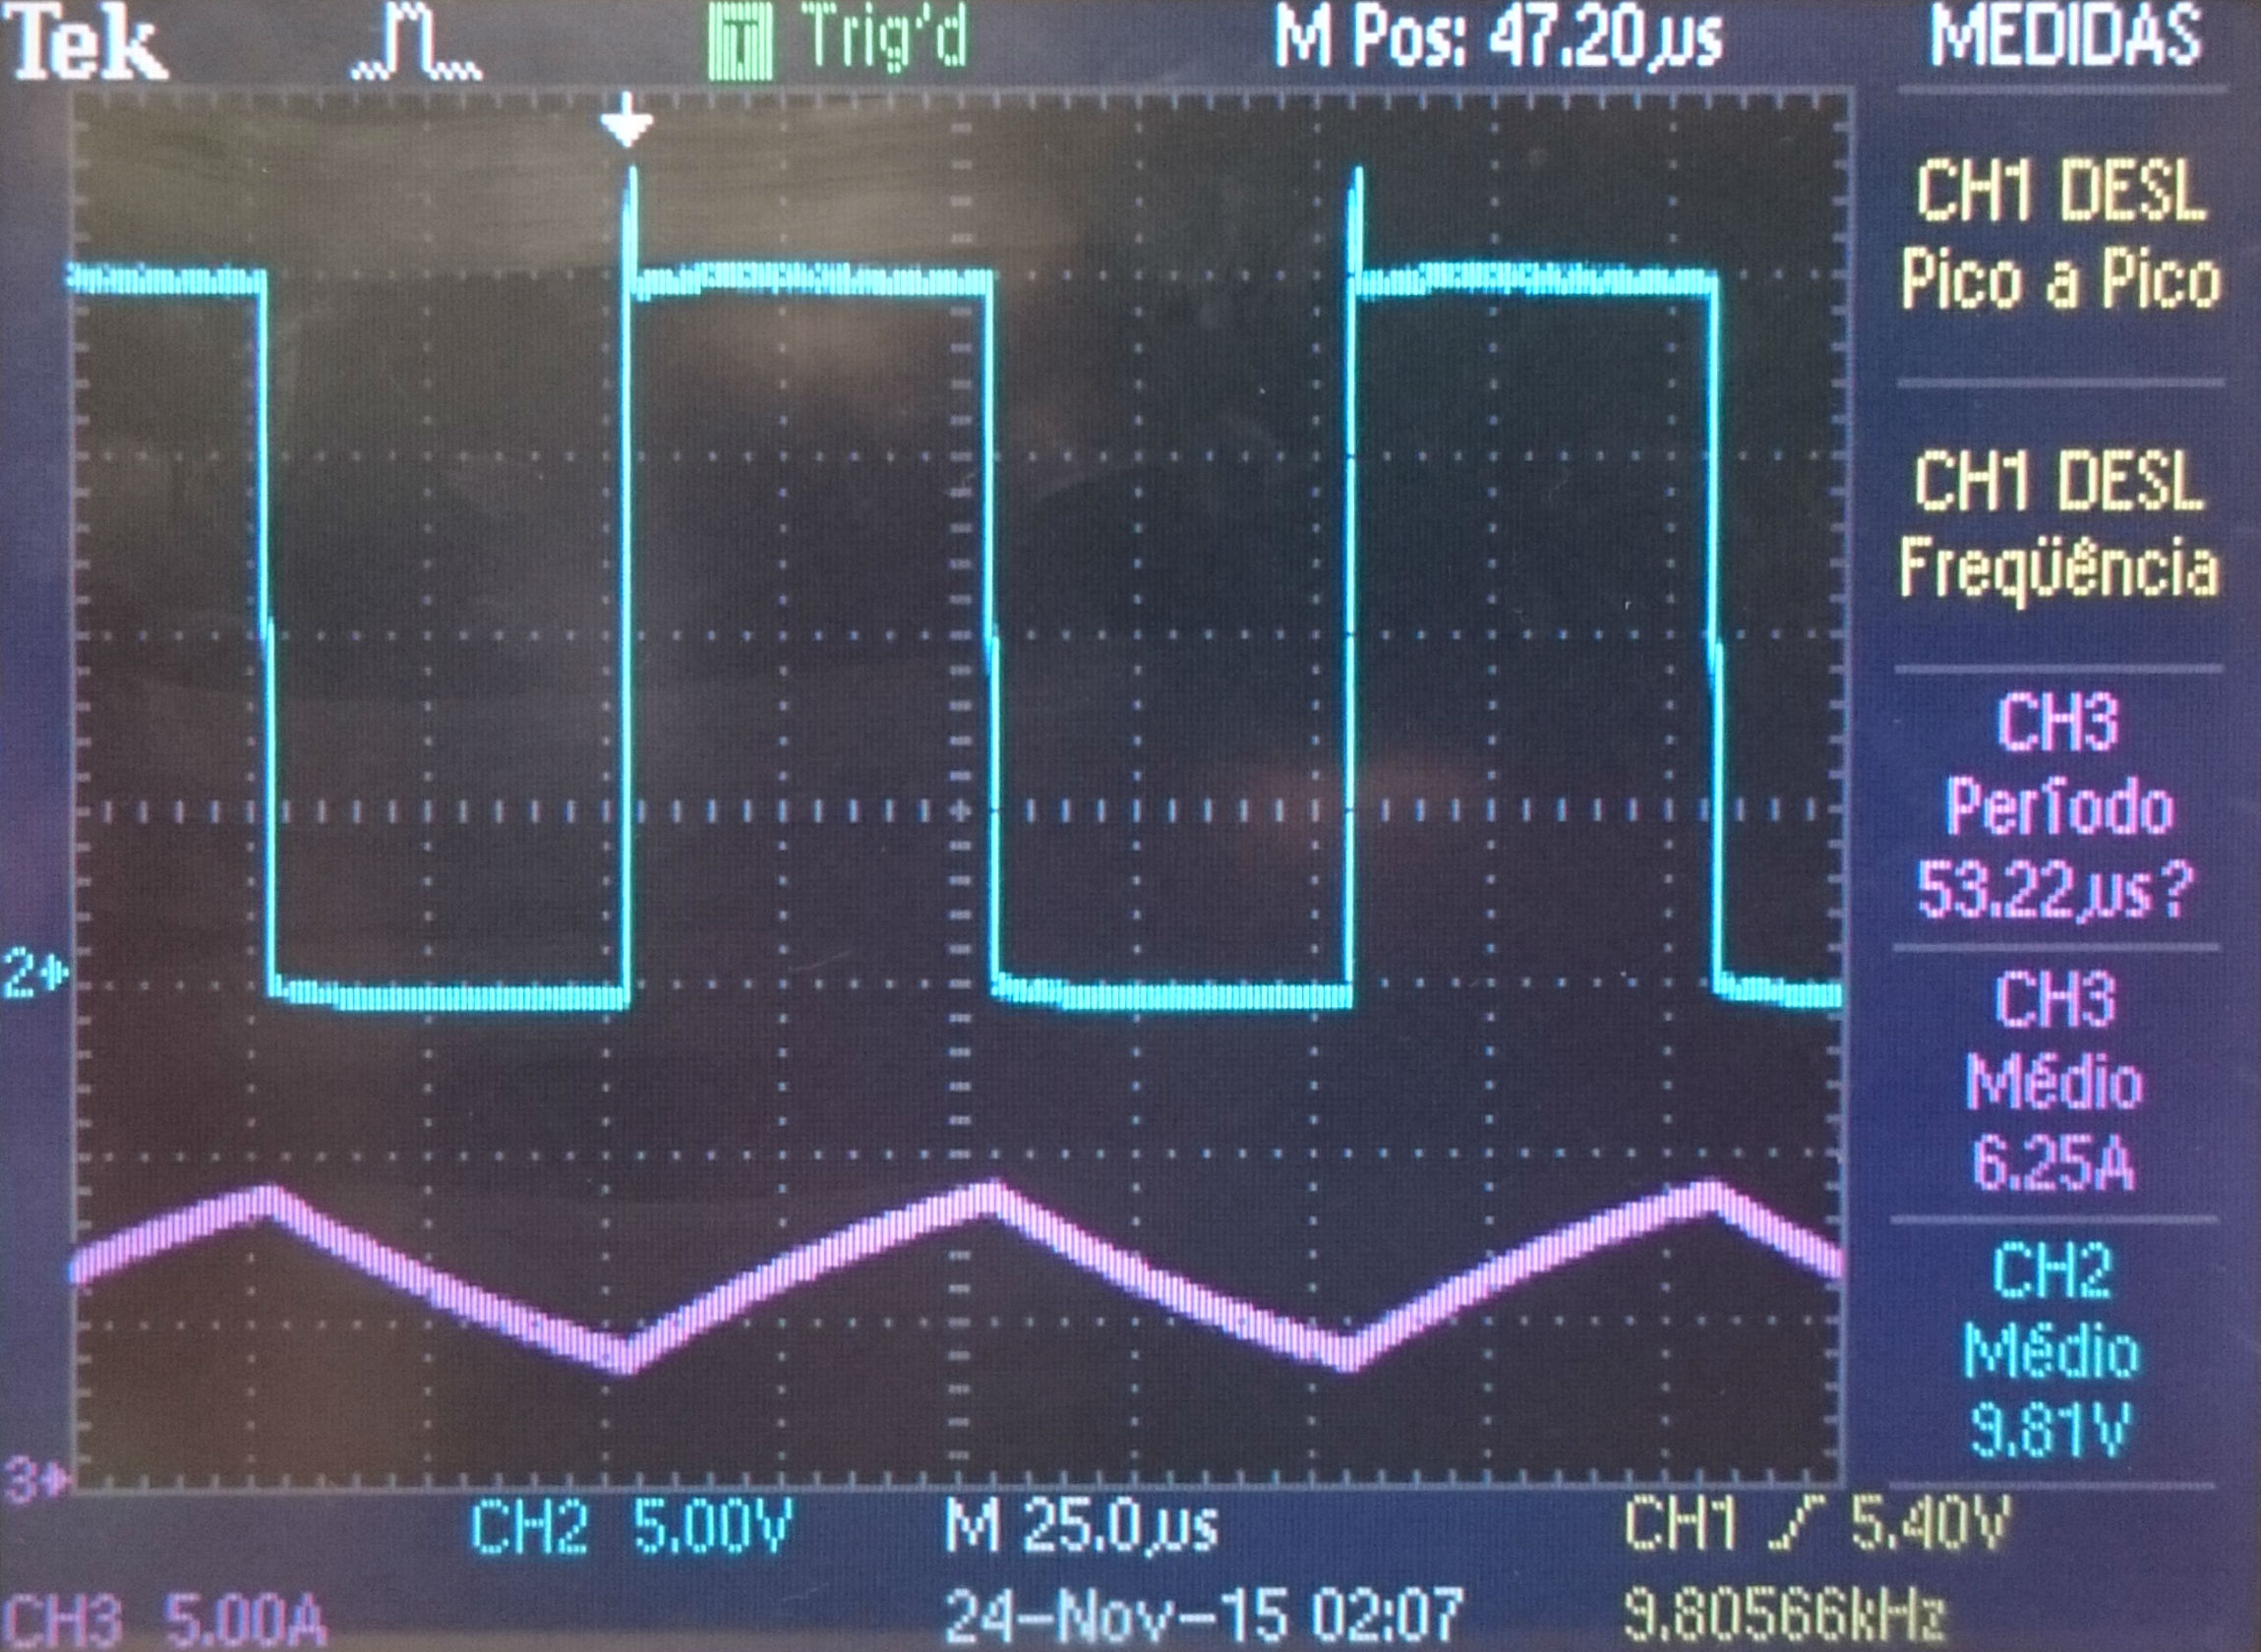
\includegraphics[keepaspectratio=true, scale=0.13]{img/figs/tensao_diodo_icarga_buckrl}
	\caption{Formas de onda da tensão aos terminais de D\textsubscript{1} e corrente na saída para Carga RL do conversor redutor.}
	\label{fig:tensao_diodo_icarga_buckrl}
	\vspace{-0.8em}
\end{figure} 

Pode ver-se a azul a tensão aos terminais do díodo e a rosa a corrente na carga.

Através da \autoref{fig:tensao_diodo_icarga_buckrl} fica evidenciado o comportamento do circuito. Nota-se que quando o transistor MOSFET está ao corte, o díodo estará consequentemente à condução, pelo que a bobine irá carregar. No instante em que o MOSFET passa à condução, o díodo D\textsubscript{1} estará ao corte e a bobine irá descarregar. 

Este processo de carga e descarga da bobine produz um \textit{ripple} na corrente de saída que está diretamente ligado com a frequência de comutação e o tamanho da bobine; naturalmente é de interesse que este \textit{ripple} seja tão reduzido quanto possível, o que implica jogar com as duas restrições já mencionadas.

\paragraph{Frequência limiar do regime lacunar}\mbox{}\

O regime lacunar observa-se quando se tem uma frequência de comutação tal, que a bobina descarrega até que a corrente caia até zero.

Embora não se tenha tirado este valor no laboratório e a figura correspondente, \todo{mencionar qual a figura da simulação} ao fazer a simulação do circuito em estudo observou-se que a frequência limite para o regime lacunar seria próxima de $4$ kHz.

\subsubsection{Carga RLC}

Para finalizar o estudo do conversor redutor, estudou-se o seu comportamento para uma carga RLC, colocando-se em paralelo com a resistência e bobina o condensador C6.

\paragraph{Formas de onda da tensão V\textsubscript{DS} e corrente I\textsubscript{D} para $20$ kHz}\mbox{}\

O pretendido era observar as formas de onda da tensão V\textsubscript{DS} e corrente I\textsubscript{D}. No entanto durante o laboratório o lido foi tal como se apresenta na \autoref{fig:vds_id_buckrlc}.

\begin{figure}[H]
	\centering
	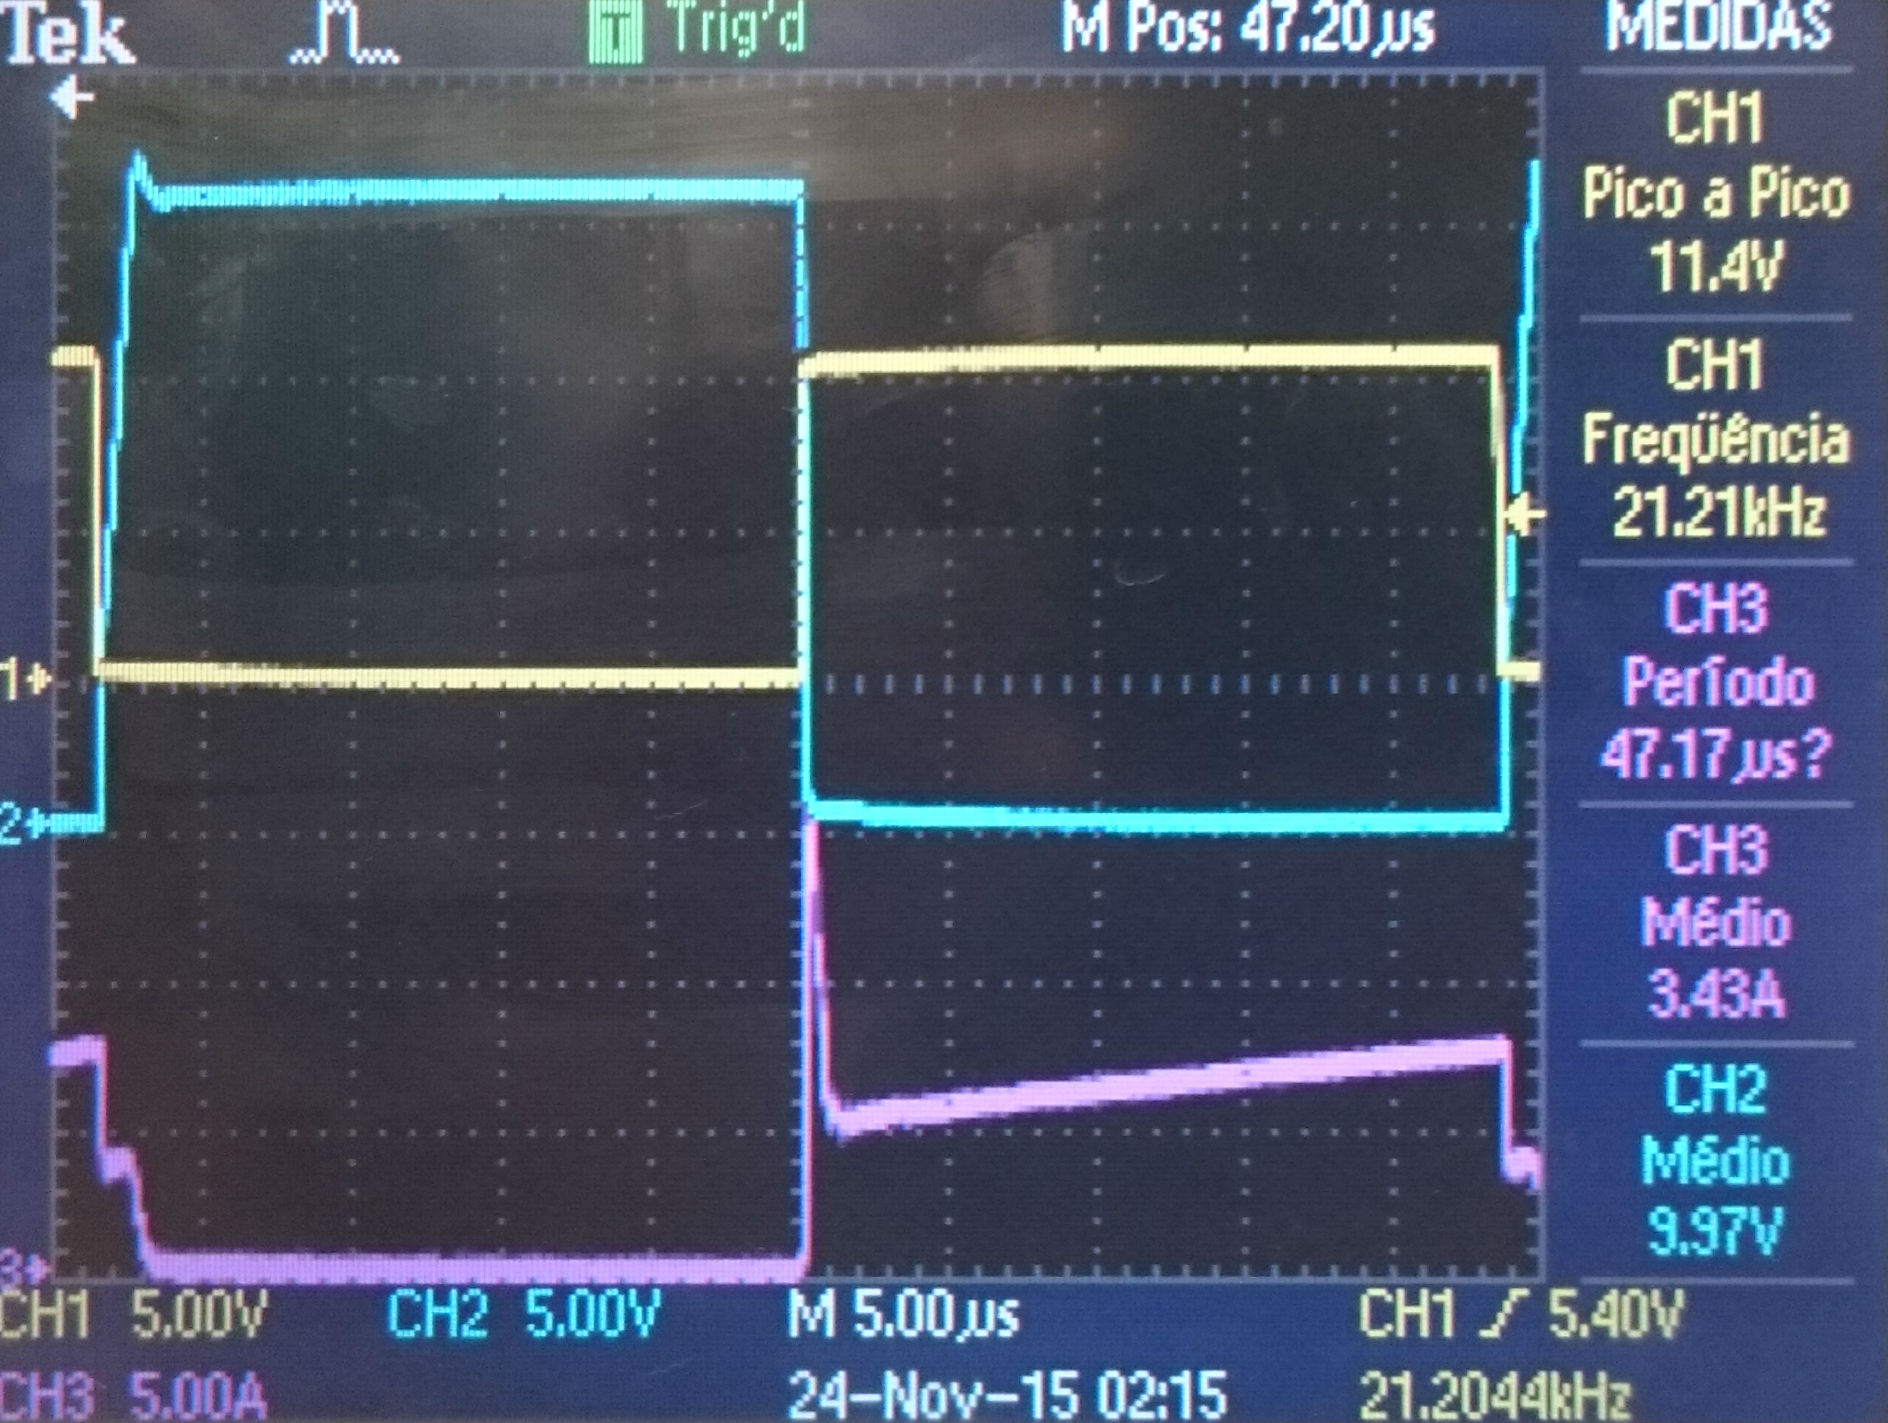
\includegraphics[keepaspectratio=true, scale=0.17]{img/figs/vds_id_buckrlc}
	\caption{Formas de onda da tensão V\textsubscript{DS} e corrente I\textsubscript{D}.}
	\label{fig:vds_id_buckrlc}
	\vspace{-0.8em}
\end{figure} 

Aqui observa-se a azul a tensão na carga, a amarelo a tensão V\textsubscript{DS} e a rosa a corrente de dreno I\textsubscript{D}.

Tendo em conta que o Díodo apenas está a conduzir quando o MOSFET está ao corte, nota-se que a tensão na saída é zero quando o transistor está ON e o contrário quando OFF; tal como se observa para os sinais a amarelo e azul na \autoref{fig:vds_id_buckrlc}.

A rosa tem-se, tal como já foi dito, a corrente I\textsubscript{D}, sendo esta a mesma que irá carregar a bobine enquanto o MOSFET está a conduzir e o díodo ao corte.

\paragraph{Formas de onda da tensão e corrente no Díodo D\textsubscript{1}}\mbox{}\

Infelizmente não se obteve as formas de onda pretendidas nesta secção no entanto conhecendo o comportamento do conversor elas são conhecidas.

A tensão aos terminais do díodo é tal como se observa a azul na \autoref{fig:vds_id_buckrlc}, fora alguma possível queda de tensão na bobine, e a corrente neste é a complementar do que se observa a rosa na mesma figura.

Esta corrente irá apresentar o mesmo valor médio que I\textsubscript{D}, no entanto como apenas irá haver corrente a percorrer no díodo quando o transistor MOSFET está ao corte, os períodos em que esta será diferente de zero serão os mesmos em que a corrente de dreno é zero. Observa-se ainda que enquanto que I\textsubscript{D} corresponde ao carregamento da bobine, a corrente que atravessa o díodo corresponde à descarga, pelo que o seu declive será negativo.

\paragraph{Formas de onda da tensão na carga e corrente na bobine}\mbox{}\

\begin{figure}[H]
	\centering
	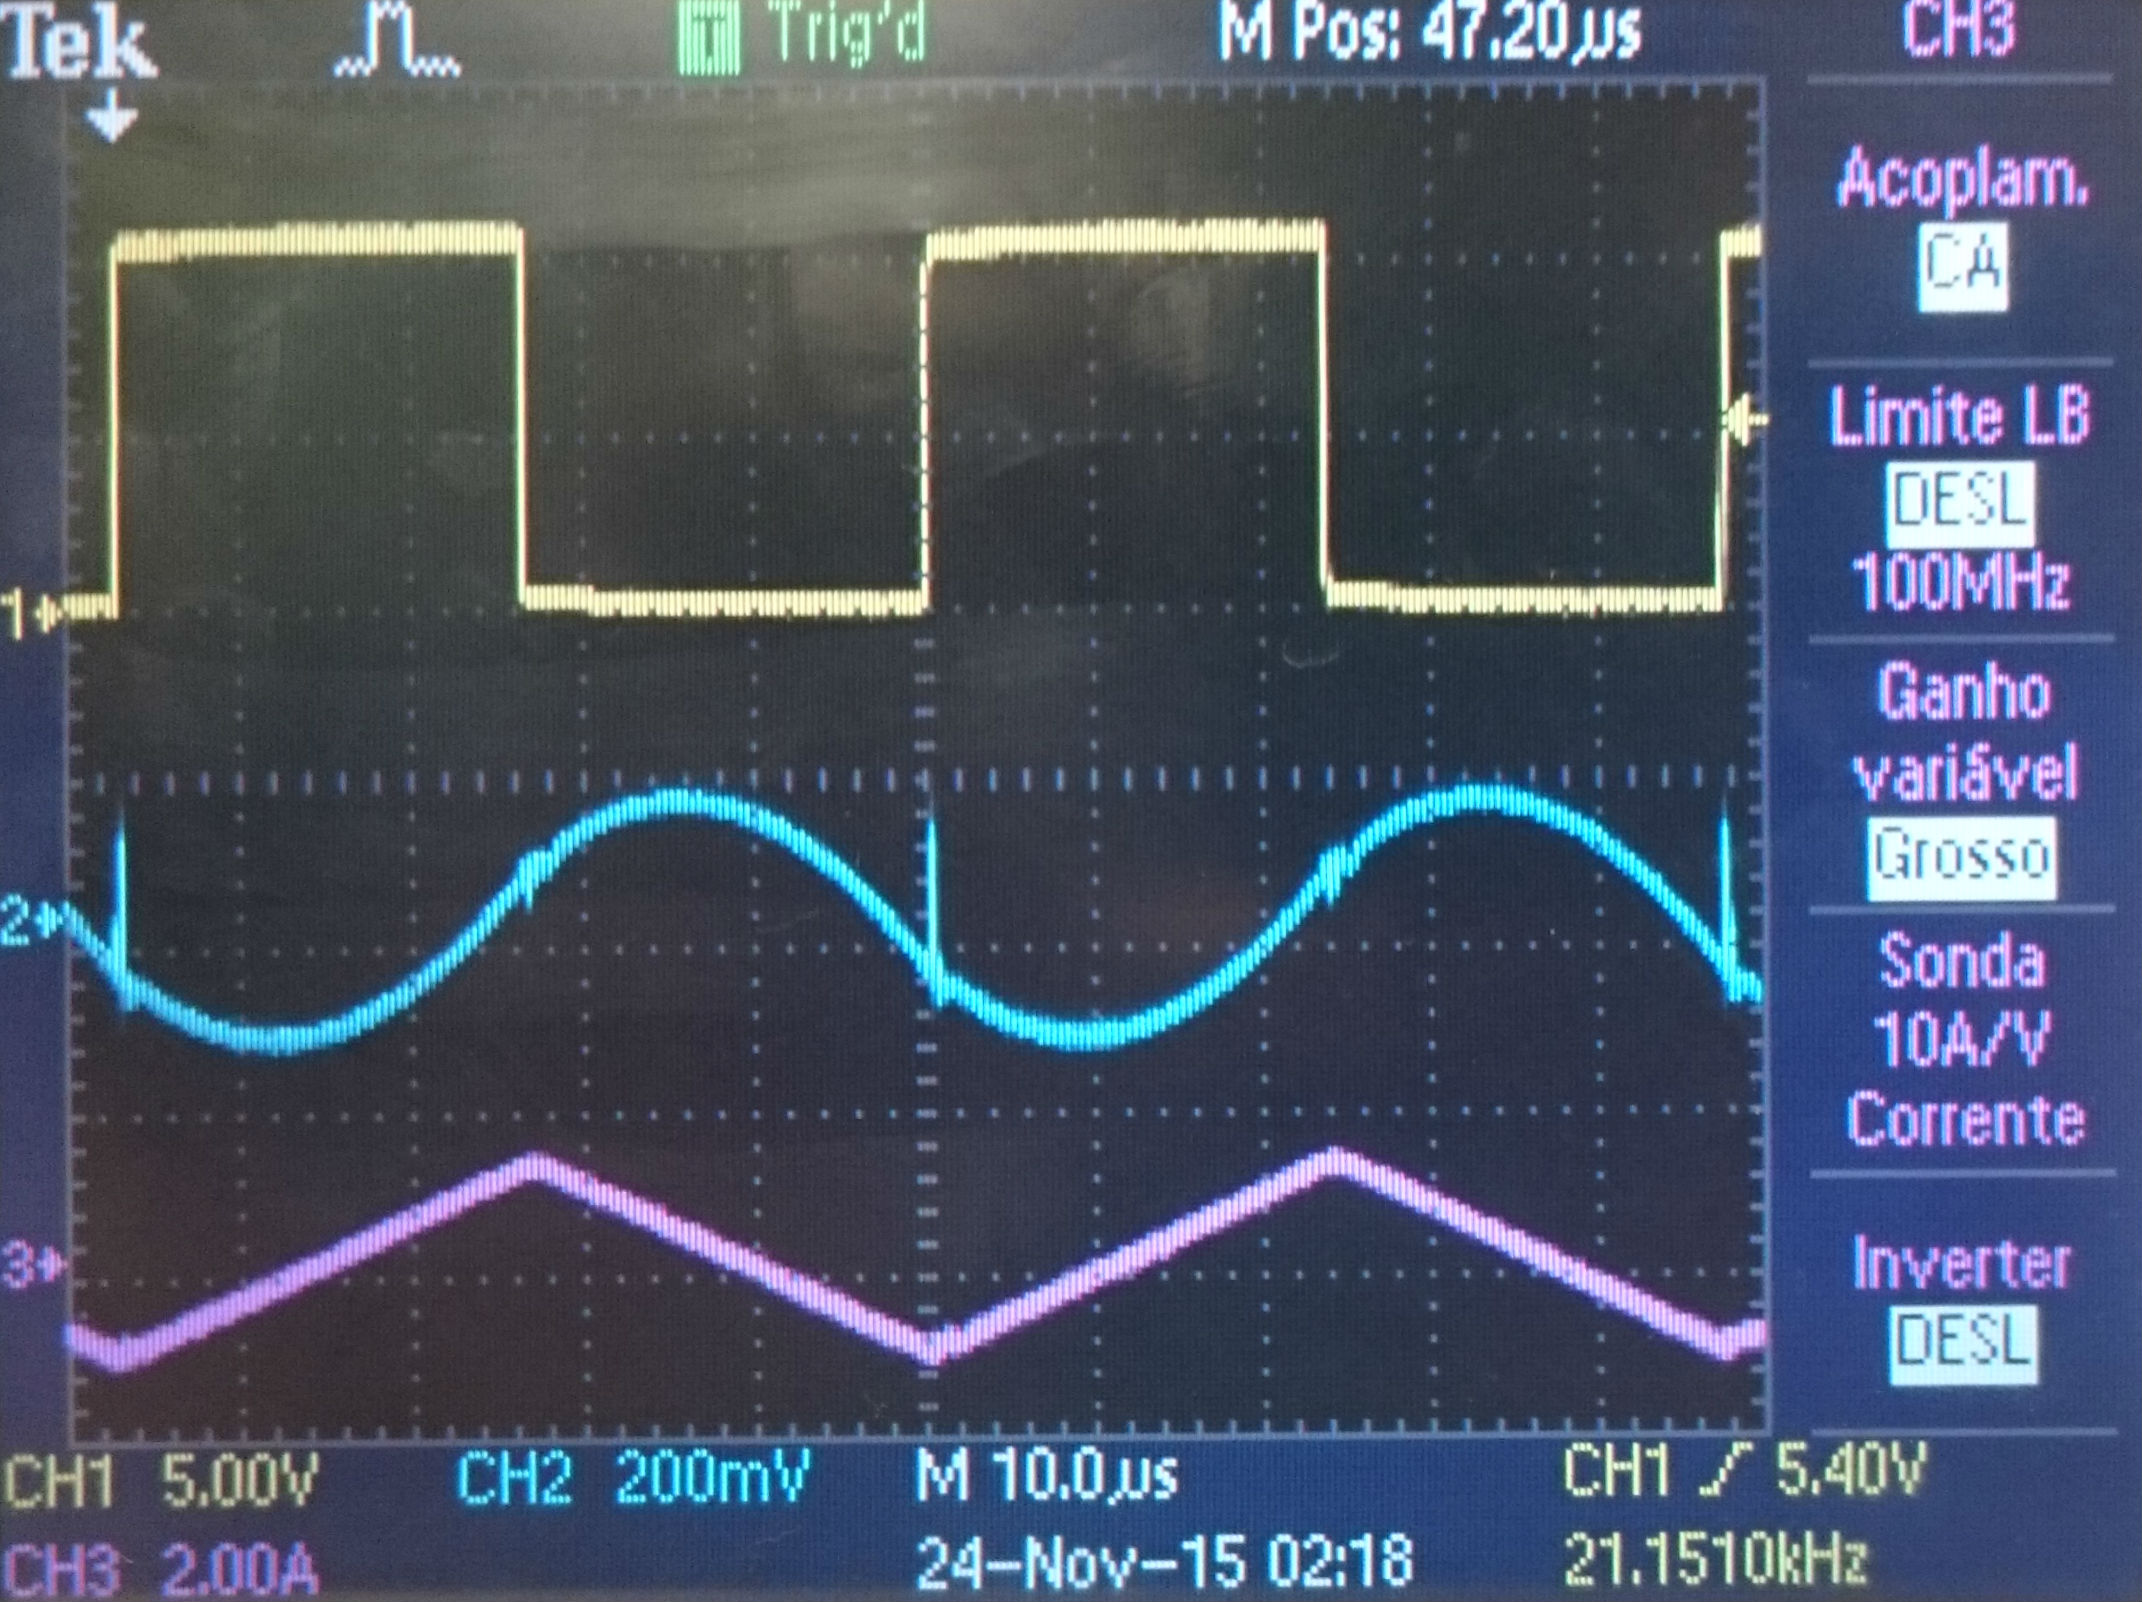
\includegraphics[keepaspectratio=true, scale=0.15]{img/figs/tensao_carga_corrente_bobine_ac_rlcbuck}
	\caption{Formas de onda da tensão e corrente na bobine.}
	\label{fig:tensao_carga_corrente_bobine_ac_rlcbuck}
	\vspace{-0.8em}
\end{figure} 

\unsure{caption}

Observa-se a amarelo a tensão V\textsubscript{DS} e a tensão e corrente aos terminais da bobine a azul e rosa respetivamente.

A partir desta figura pode compreender-se bem o comportamento do conversor redutor sujeito a uma carga RLC. Tem-se que durante o período em que o MOSFET está em condução, o díodo estará ao corte e a bobine carrega; observável pelo declive crescente da corrente na saída. 

Quando o MOSFET passa ao corte, o díodo passa à condução pelo que a bobine começa a descarregar; sendo que se tem corrente com declive negativo. Como o observado a rosa é a corrente na bobina, tem-se um valor médio desta igual a zero, tal como esperado quando se está a lidar com este componente, e nota-se também que o valor médio da tensão aos seus terminais é igualmente zero.

\paragraph{Tensão na carga em função do fator de ciclo}\mbox{}\

O fator de ciclo relaciona a tensão de entrada com a de saída e a sua expressão para o conversor redutor é conhecida e tal como se apresenta na \autoref{D_buck}.

\begin{equation}
	D= \frac{V_o}{V_i} \label{D_buck}
\end{equation}

Sendo assim, fazendo variar o fator de ciclo, e conhecendo o valor da tensão de entrada, que é imposto como igual a $20$ V, pode então obter-se o valor teórico para a tensão de saída através da \autoref{Vo_buck}.

\begin{equation}
V_o= \frac{D}{V_i} \label{Vo_buck}
\end{equation}

Sendo assim pode fazer-se uma comparação entre os valores esperados teoricamente e os lidos no laboratório, estando esta comparação presente na \autoref{tab:tabela_buck}

\begin{table}[!htb]
	\centering
	\caption{Comparação entre valores teóricos e experimentais da tensão de saída em função do fator de ciclo.}
	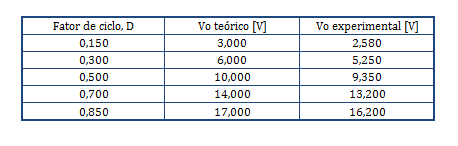
\includegraphics[width=0.8\linewidth]{teoricas/tabela_buck}
	\label{tab:tabela_buck}
\end{table}

Para que seja possível observar esta relação de forma mais expedita, apresenta-se também um gráfico para a mesma, visível na \autoref{fig:graf_buck}

\begin{figure}[H]
	\centering
	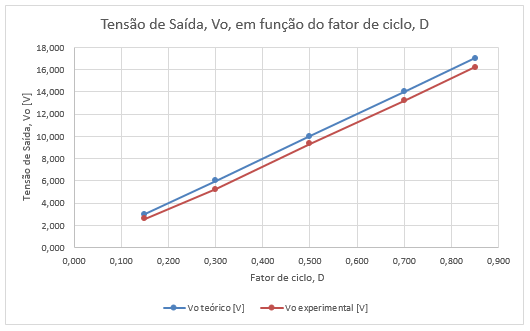
\includegraphics[keepaspectratio=true, scale=1.0]{teoricas/graf_buck}
	\caption{Gráfico de comparação entre valores teóricos e experimentais da tensão de saída em função do fator de ciclo.}
	\label{fig:graf_buck}
	\vspace{-0.8em}
\end{figure}

Observa-se assim que através do fator de ciclo é possível controlar o grau de atenuação da tensão de saída face à de entrada, estando o conversor a funcionar tal como desejado, ou seja, um "transformador" redutor de tensão DC.

Nota-se no entanto uma ligeira diferença entre o valor teórico e o experimental, que se deve essencialmente a possíveis perdas e não idealidades dos componentes semicondutores, que não estão consideradas na aplicação da \autoref{D_buck}.

\paragraph{Efeito de um \textit{Snubber} entre o Dreno e \textit{Source} do MOSFET para $50$ kHz}\mbox{}\

De seguida aumentou-se a frequência para que fosse possível evidenciar o efeito do \textit{Snubber} entre o dreno e \textit{Source} do MOSFET. As formas de onda obtidas podem ser vistas na \autoref{fig:snubber_buck}.

\begin{figure}[H]
	\centering
	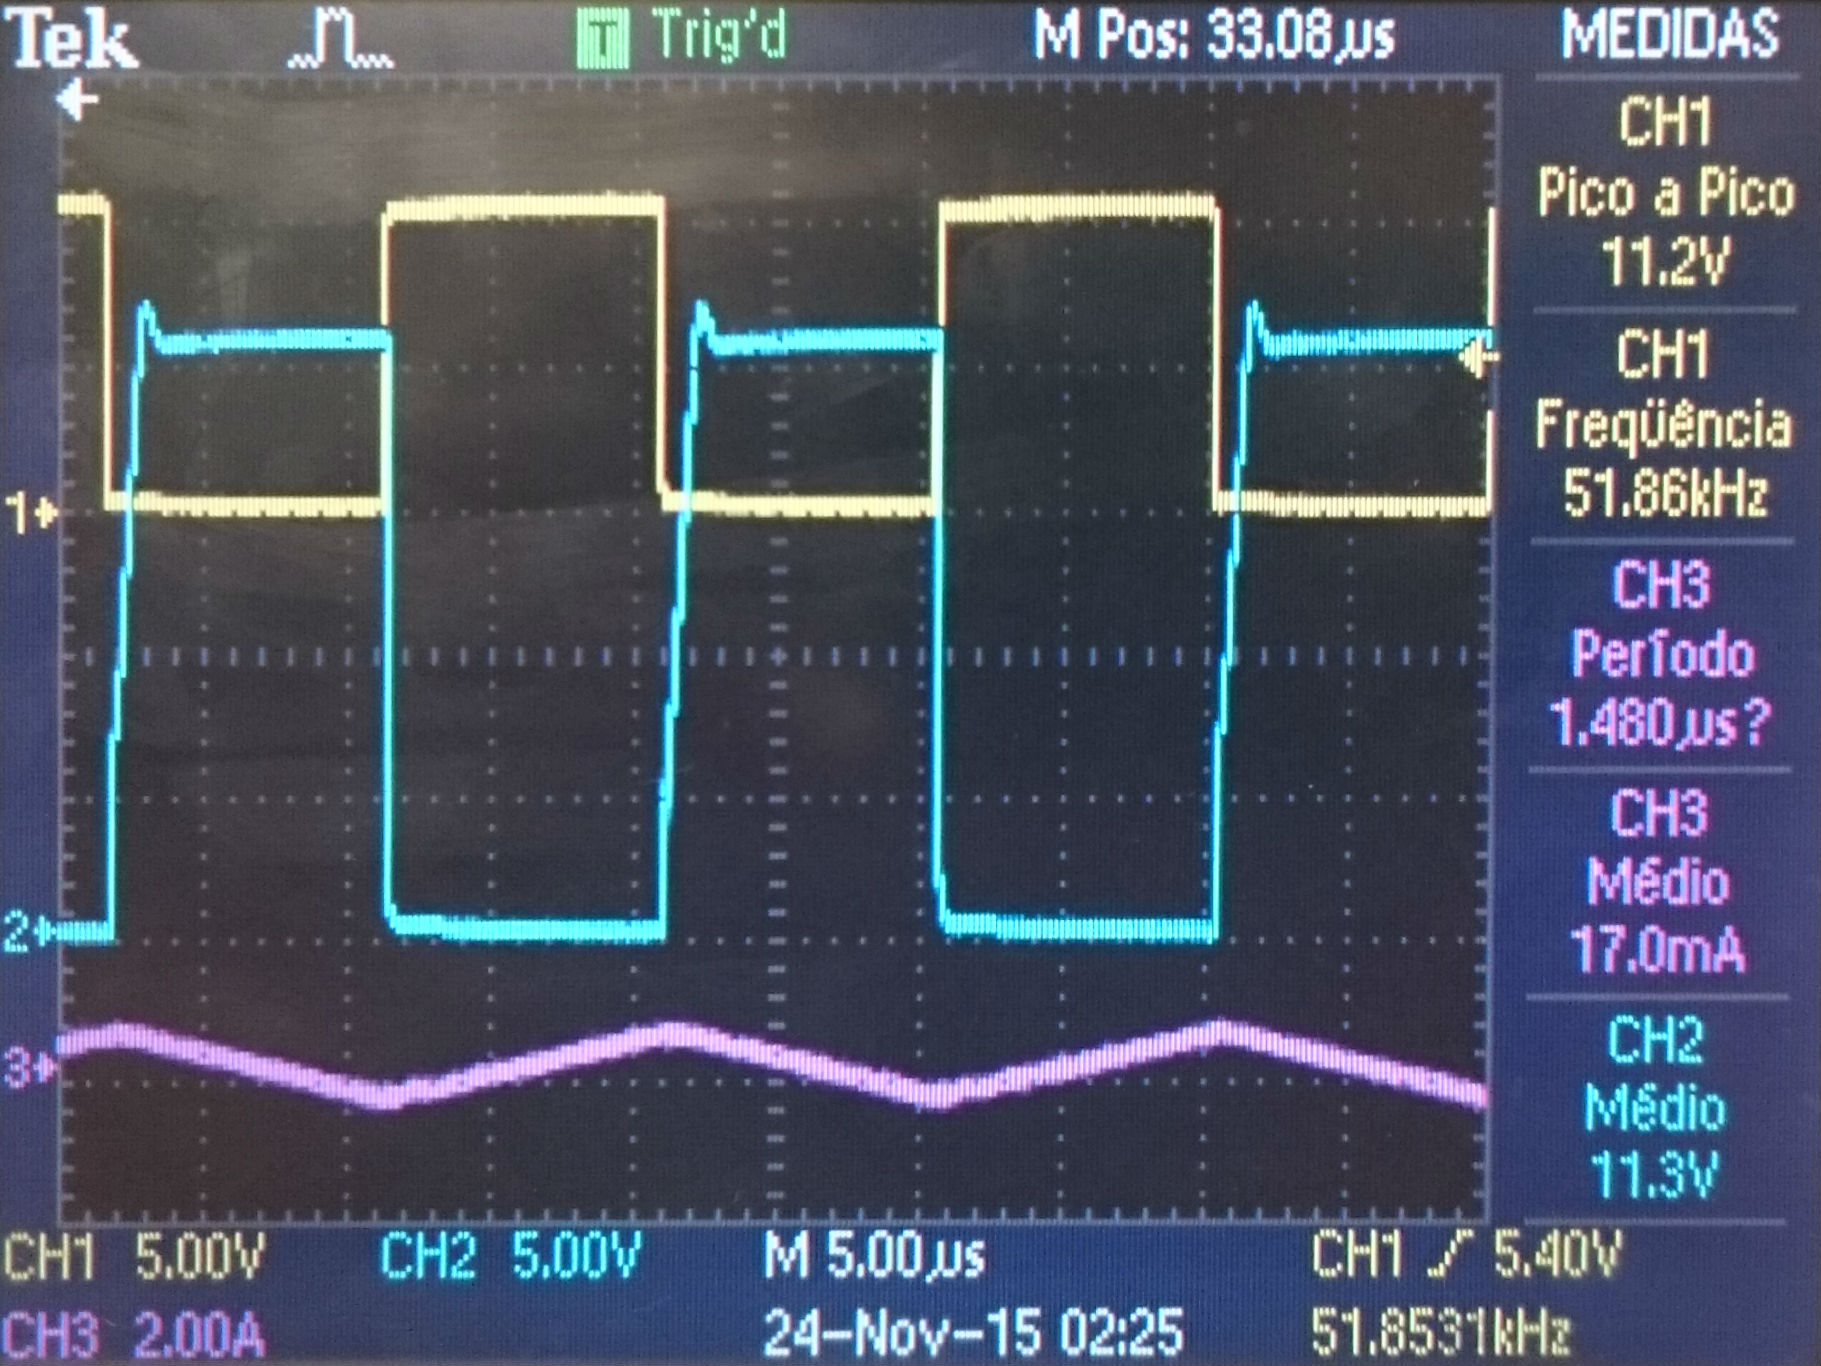
\includegraphics[keepaspectratio=true, scale=0.175]{img/figs/snubber_buck}
	\caption{Efeito de um \textit{snubber} nas formas de onda tensão de saída e corrente na bobine.}
	\label{fig:snubber_buck}
	\vspace{-0.8em}
\end{figure}

Nesta pode ver-se a amarelo a tensão aos termianis do MOSFET, a azul a tensão na carga e a rosa a corrente na bobine.

Com a presença do \textit{snubber} pretende-se um efeito idêntico ao de um filtro passa baixo, para que seja possível eliminar os picos de alta frequência na tensão. Nota-se no entanto por observação da figura que o efeito é marginal, pelo que a frequência de corte do \textit{snubber}
deverá ser superior à de operação considerada.

\paragraph{Forma de onda da tensão V\textsubscript{AK} do Díodo D\textsubscript{1} para $200$ kHz}\mbox{}\

Na sequência da subsecção anterior aumentou-se a frequência de operação para $200$ kHz sendo as formas de onda obtidas apresentadas na \autoref{fig:vak_hf_buck}.

\begin{figure}[H]
	\centering
	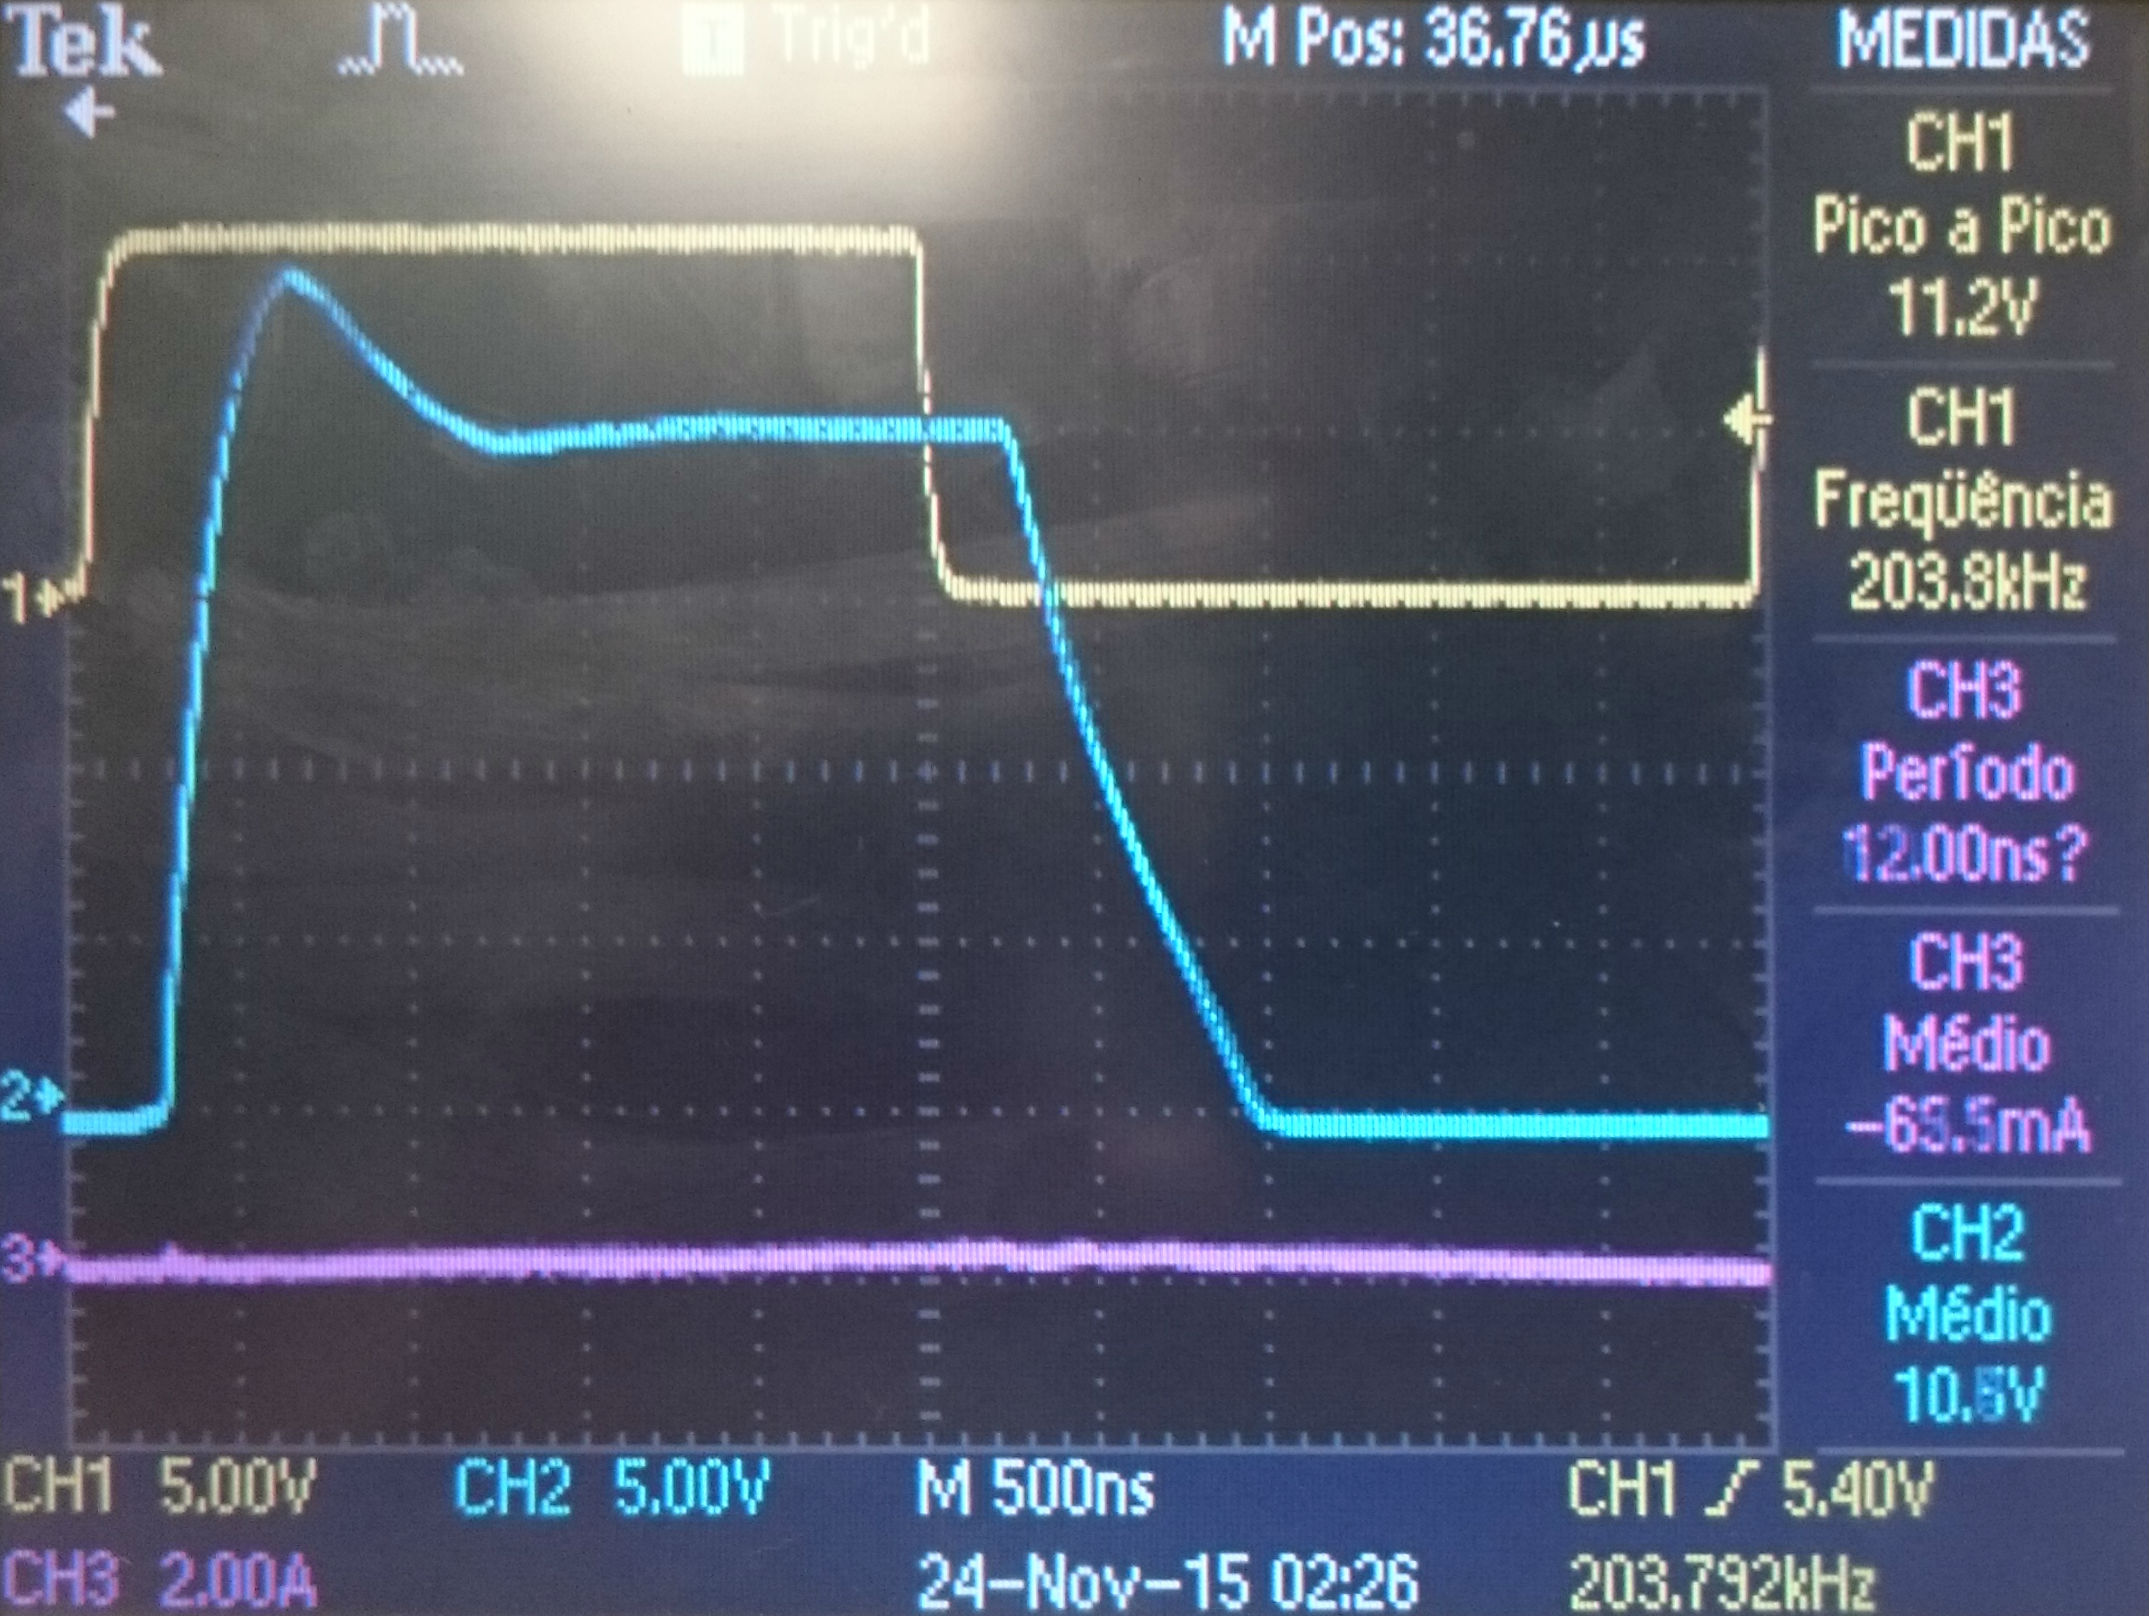
\includegraphics[keepaspectratio=true, scale=0.175]{img/figs/vak_hf_buck}
	\caption{Formas de onda da tensão V\textsubscript{AK} do Díodo D\textsubscript{1} para $200$ kHz.}
	\label{fig:vak_hf_buck}
	\vspace{-0.8em}
\end{figure}

Novamente a amarelo tem-se a tensão aos termianis do MOSFET, a azul a tensão aos terminais do díodo e a rosa a corrente na bobine.

Pode ver-se agora que a frequência do pico da tensão no díodo será bastante inferior pelo que esta frequência de operação estará próxima da de corte do \textit{snubber}, pelo que o seu efeito já é apreciável nesta situação.

\subsection{Conversor Ampliador}

\paragraph{Formas de onda da tensão V\textsubscript{DS} e da corrente I\textsubscript{D} para $40$ kHz}\mbox{}\

\paragraph{Formas de onda na Resistência e corrente em D\textsubscript{1}}\mbox{}\

\paragraph{Tensão na carga em função do fator de ciclo}\mbox{}\

\subsection{Converor Redutor-Ampliador}

\paragraph{Formas de onda da tensão e corrente aos terminais da bobina para $40$ kHz}\mbox{}\

\paragraph{Formas de onda da tensão na Resistência e corrente D\textsubscript{1}}\mbox{}\

\paragraph{Tensão na carga em função do fator de ciclo}\mbox{}\

\paragraph{Rendimento do conversor para um fator de ciclo de $60$ \%}\mbox{}\

\pagebreak

\begin{thebibliography}{2}
	
	\bibitem{Kassakian}
	Kassakian, John G. et al (1992, June), Principles of Power Electronics, \textit{Addison-Wesley Publishing Company}

	\bibitem{Rashid}
	Rashid, Muahammad H. (2004), Power Electronics - Circuits, Devices and Applications, \textit{Prentice Hall}
	
	\bibitem{Silva}
	Silva, Fernando (1998), Eletrónica Industrial, Fundação Calouste Gulbenkian
	
\end{thebibliography}


\pagebreak



\end{document}
